% !TEX root = thesis-thomas-tiotto.tex

\section{Data set}
As anticipated in Chap. \ref{chap:introduction} the work carried out in this thesis had a certain degree of collaboration with a third party, \cite{istitutocantonalepresentazione}.

\subsection{Istituto Cantonale di Patologia}
Istituto Cantonale di Patologia (ICP) is an institute based in Locarno that is specialised in the histological analysis of tissue samples received from private patients, clinics and hospitals, mainly in support of cancer diagnosis.
These tests are aimed at identifying the precise profile of the cancer cells and thus inform the clinician on the best treatment for the specific patient.

In addition to its clinical support activities, the Istituto also carries out scientific research aimed at better understanding certain types of cancers at a basic level.
In the last ten years, the ICP has published more than 200 peer-reviewed papers and more than 100 works in non-peer reviewed journals and is active at a national and international level.

\subsection{Motivation}
My first contact with the ICP was during a meeting with Dr. Vittoria Martin (\cite{martin2012}), molecular citogenetist, in date 28/01/2019.
The institute had expressed interest in bringing machine learning into their workflow in order to both augment their profiling capabilities for patients and to be able to extract new knowledge from their existing data.
This knowledge-extraction may lead towards the confirmation of current scientific theories or may be the first step towards the formulation of novel ones.

\todo{chiedere a Vittoria martedì cosa si aspettavano/aspettano}

My interest in collaborating with the Istituto stemmed from the desire to apply the methods described in Sec. \ref{sec:novel-contributions} to a real-world case.
Being the theoretical work being carried out in this thesis an expert-driven MPE approximation, collaboration with the institute has also provided the opportunity to implement a proof of concept using real histological data.
The doctors and researchers of the Istituto have been able to validate the model software that I have developed from an Explainable AI point of view.
That is to say, they have validated the capacity of the developed software to support clinical decision making and surface clarifying explanations of the data set.

\todo{da confermare con Vittoria più avanti}

\subsection{Provided data set}
The data set I was provided with consists of the histological records of 3218 breast cancer patients.
The data set had been pre-processed by collaborators of the ICT with some of the values being compiled by hand. 
In Tab. \ref{tab:datasetvariables} is a description of the measured variables, together with their clinical meaning.
The value distribution of the data set is shown in Tab. \ref{tab:datasetdistribution}.

The indications from Dr. Martin on how to further preprocess the data are shown in Tab. \ref{tab:datasetpreprocess}.
Note that some variable names were simplified.


\begin{table*}[htbp]
\caption{Data set variables}
\begin{tabularx}{\textwidth}{@{} l Y @{}}
\toprule 
\textbf{Variable} & Meaning \\
\midrule 
\textbf{Codice globale} & Unique patient identifier \\
\textbf{mut17q21} & \\
\textbf{loss 17} & \\
\textbf{et\`a arrotondata} & The age of the patient at diagnosis\\
\textbf{Lateralit\`a} & The affected breast \\
\textbf{Situ SUBGROUP MZ} & The site code of the tumour \\
\textbf{Morfologia SUBGROUP MZ} & The morphology classification of the tumour \\
\textbf{pT SUBGROUP MZ} & Primary tumour in the TNM classification for breast cancer \\
\textbf{pN SUBGROUP MZ} & Pathologic in the TNM classification for breast cancer \\
\textbf{M 8.2.96} & Distant metastasis in the TNM classification for breast cancer \\
\textbf{Differenziazione} &  \\
\textbf{Recettori estrogeni percento 1.1.2003} & \\
\textbf{Recettori progestinici percento 1.1.2003} & \\
\textbf{c erbB 2  cod percento 1.1.2003} & \\
\textbf{Ki67 cod percento} & \\
\textbf{FISHRatio} & \\
\bottomrule
\end{tabularx}
\label{tab:datasetvariables}
\end{table*}

\begin{table*}[htbp]
\caption{Data set distribution}
\begin{tabularx}{\textwidth}{@{} l X c @{}}
\toprule 
\textbf{Variable} & Unique values & Distribution \\
\midrule 
\textbf{mut17q21} & 2 & 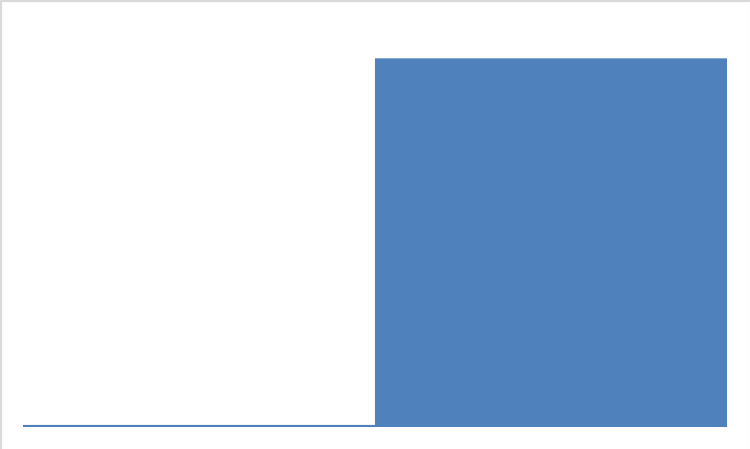
\includegraphics[width=0.2\textwidth, height=10mm]{methodology/images/mut17q21}  \\
\textbf{loss 17} & 3 & 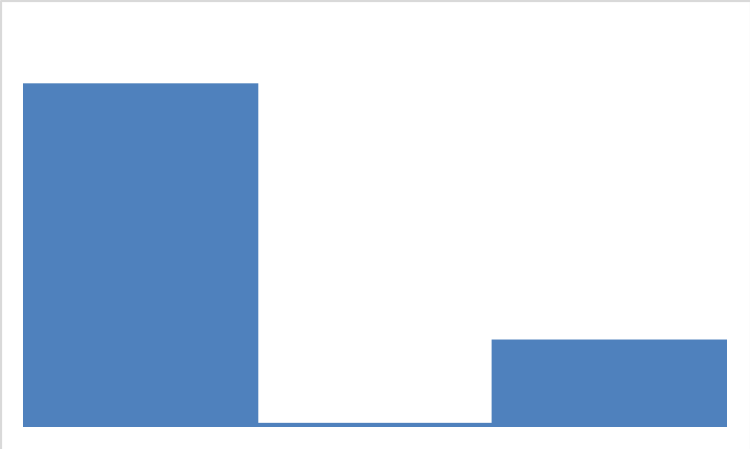
\includegraphics[width=0.2\textwidth, height=10mm]{methodology/images/loss_17}\\
\textbf{eta arrotondata} & 74 & 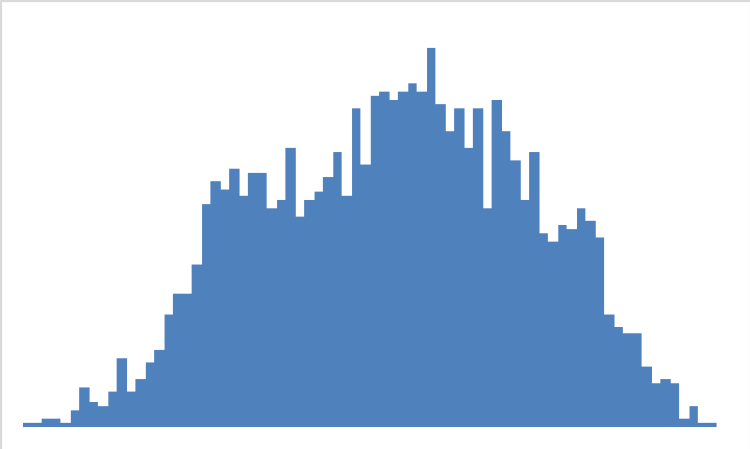
\includegraphics[width=0.2\textwidth, height=10mm]{methodology/images/eta_arrotondata}\\
\textbf{ateralit\`a} & 3 & 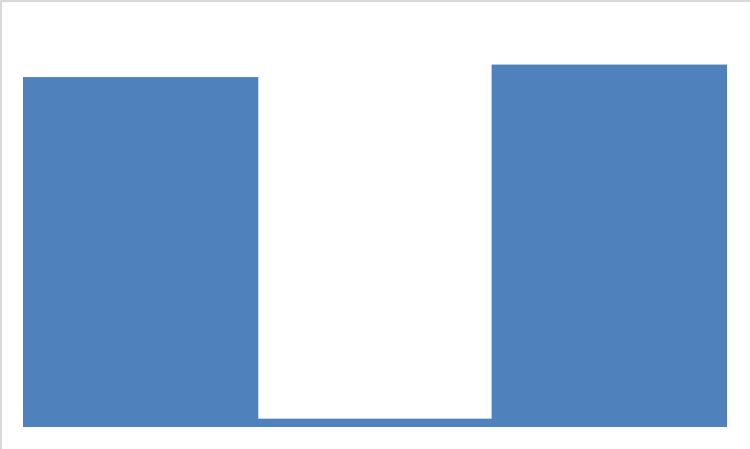
\includegraphics[width=0.2\textwidth, height=10mm]{methodology/images/lateralita} \\
\textbf{situ} & 5 & 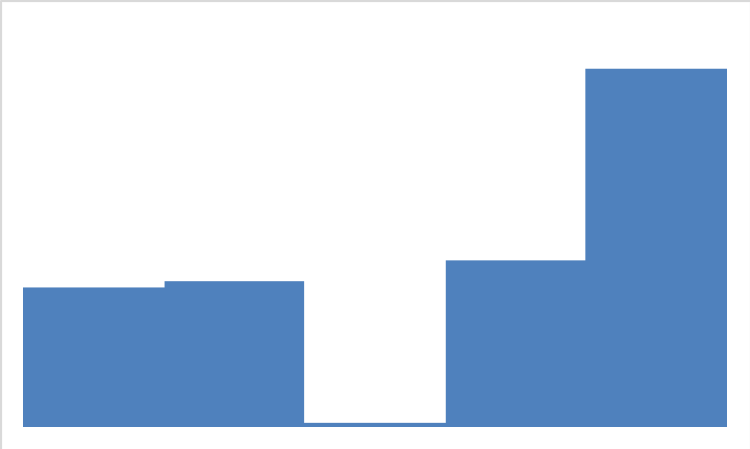
\includegraphics[width=0.2\textwidth, height=10mm]{methodology/images/situ} \\
\textbf{morfologia} & 5 & 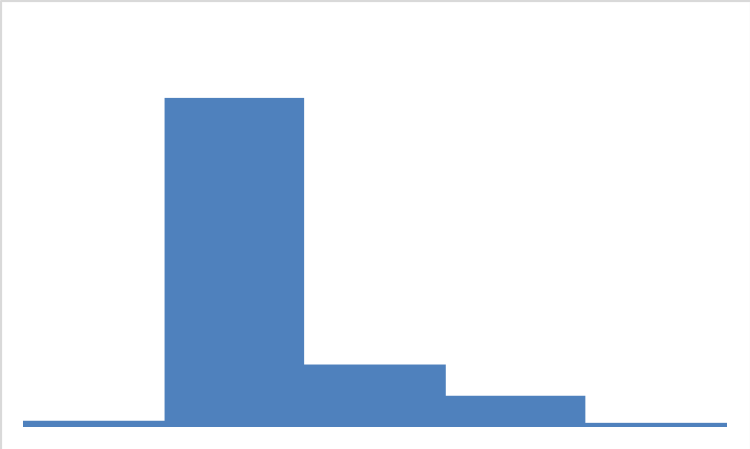
\includegraphics[width=0.2\textwidth, height=10mm]{methodology/images/morfologia} \\
\textbf{pT} & 23 & 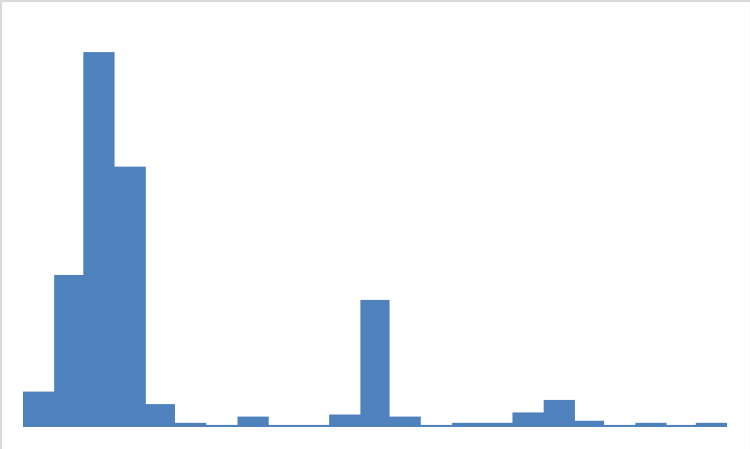
\includegraphics[width=0.2\textwidth, height=10mm]{methodology/images/pt} \\
\textbf{pN} & 6 & 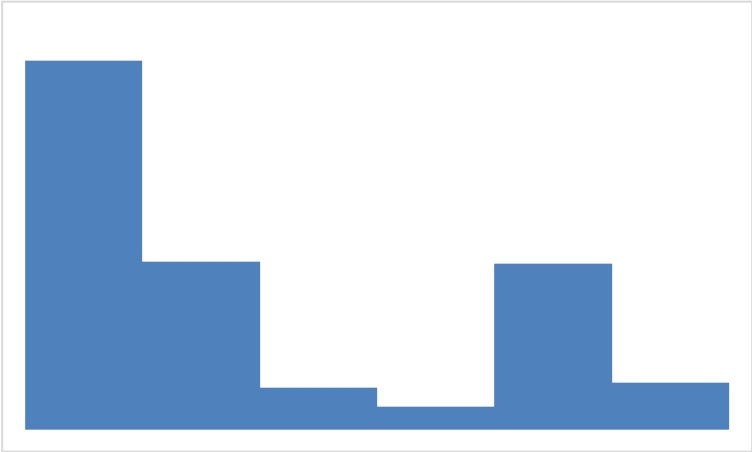
\includegraphics[width=0.2\textwidth, height=10mm]{methodology/images/pn} \\
\textbf{M} & 3 & 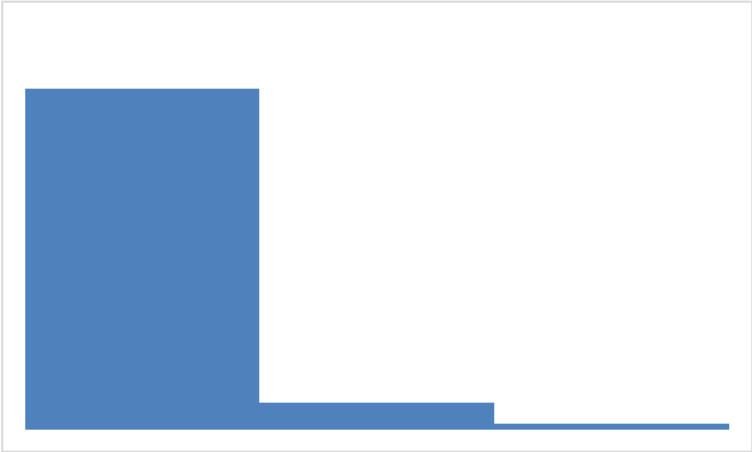
\includegraphics[width=0.2\textwidth, height=10mm]{methodology/images/m} \\
\textbf{differenziazione} & 5 & 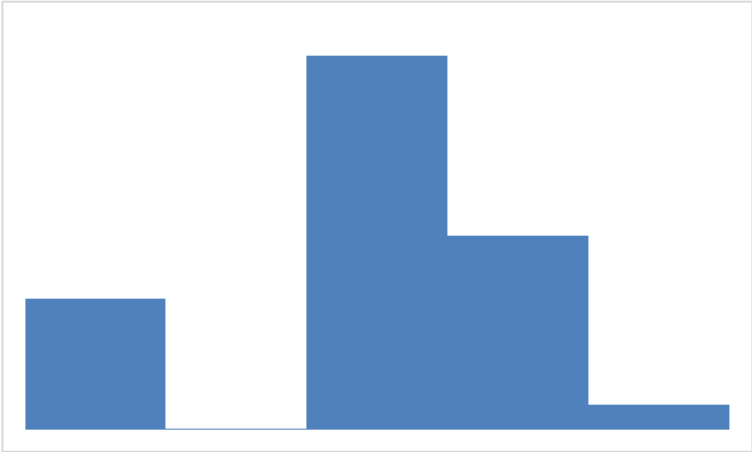
\includegraphics[width=0.2\textwidth, height=10mm]{methodology/images/differenziazione}  \\
\textbf{recettori estrogeni} & 40 & 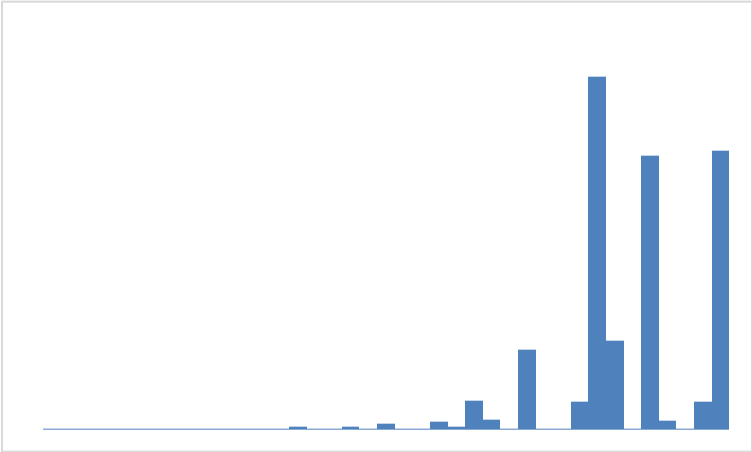
\includegraphics[width=0.2\textwidth, height=10mm]{methodology/images/recettori_estrogeni} \\
\textbf{recettori progestinici} & 40 & 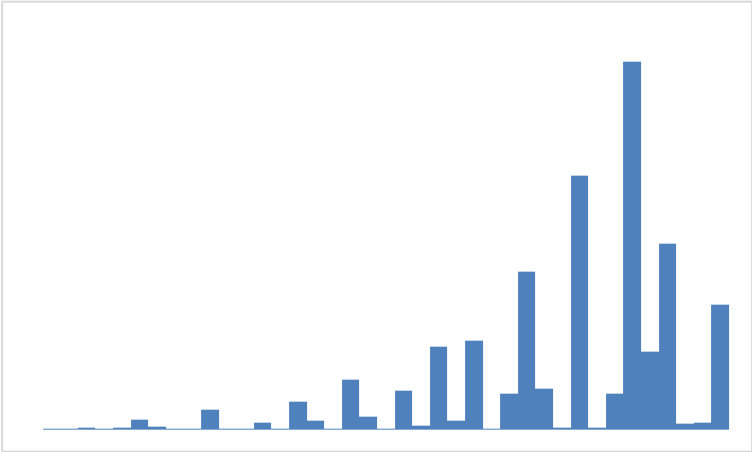
\includegraphics[width=0.2\textwidth, height=10mm]{methodology/images/recettori_progestinici}\\
\textbf{c erbB 2} & 4 & 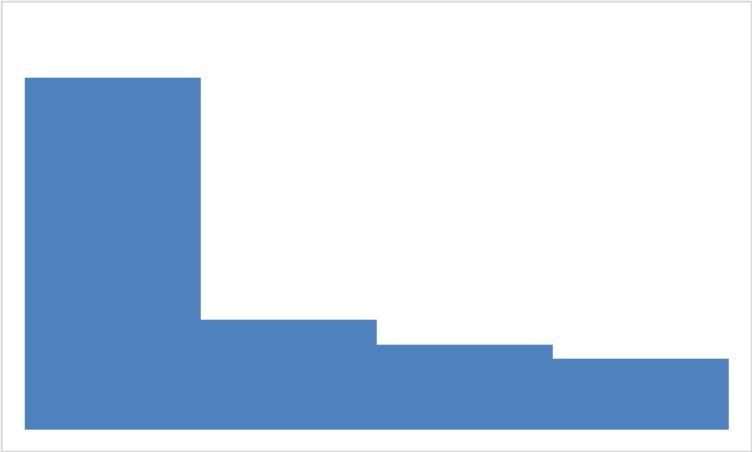
\includegraphics[width=0.2\textwidth, height=10mm]{methodology/images/c_erb_2}\\
\textbf{Ki67} & 52 & 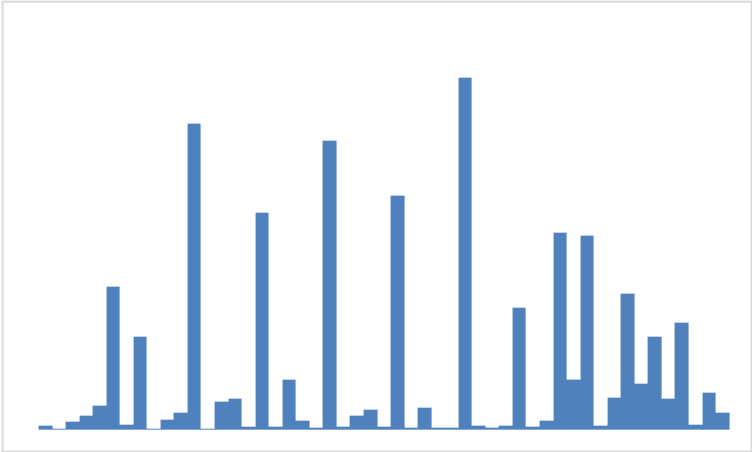
\includegraphics[width=0.2\textwidth, height=10mm]{methodology/images/ki67}\\
\textbf{FISH} & 5 & 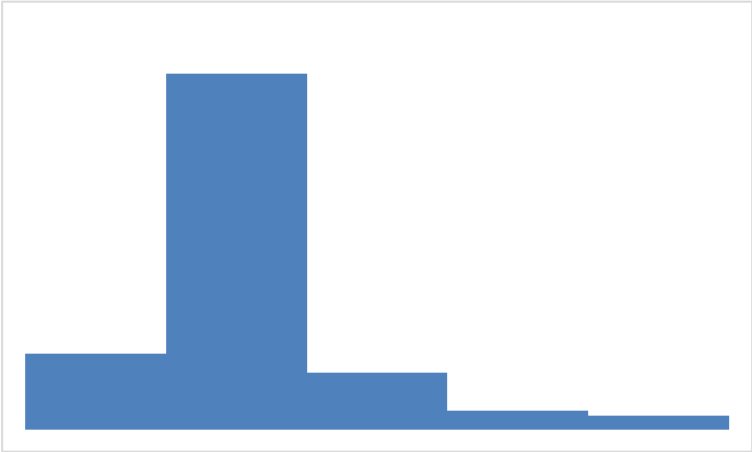
\includegraphics[width=0.2\textwidth, height=10mm]{methodology/images/fish}\\
\bottomrule
\end{tabularx}
\label{tab:datasetdistribution}
\end{table*}

\begin{table*}[htbp]
\caption{Data set preprocessing}
\begin{tabularx}{\textwidth}{@{} l Y @{}}
\toprule 
\textbf{Variable} & Action \\
\midrule 
\textbf{Codice globale} & Remove variable \\
\textbf{mut17q21} & Remove blanks \\
\textbf{loss 17} & Remove blanks \\
\textbf{eta arrotondata} & Bin into \enquote{$< 40$}, \enquote{$40-50$}, \enquote{$\geq 50$}\\
\textbf{lateralita} & Remove blanks and \enquote{sconosciuta} \\
\textbf{situ} & Remove blanks \\ \addlinespace
\textbf{morfologia} & Remove blanks and \enquote{unuseful} if performance on classification is subpar \\ \addlinespace
\textbf{pT} & Remove blanks and \enquote{unuseful}  \\
\textbf{pN} & Remove blanks and bin into \enquote{0} and \enquote{$\neq0$}\\
\textbf{M} & Remove blanks \\ 
\textbf{differenziazione} & Remove blanks and \enquote{Sconosciuto o non applicabile} \\ \addlinespace
\textbf{recettori estrogeni} & Remove blanks and bin into \enquote{negativo} if $\leq 10$,
		\enquote{debolmente positivo} if $\leq 50$, 
		\enquote{fortemente positivo} if $> 50$ \\ \addlinespace
\textbf{recettori progestinici} & Remove blanks and bin into \enquote{negativo} if $\leq 10$, 
		\enquote{debolmente positivo} if $\leq 50$, 
		\enquote{fortemente positivo} if $> 50$ \\ \addlinespace
\textbf{c erbB 2} & Remove blanks \\ 
\textbf{ki67} & Remove blanks and bin into \enquote{<14}, 
		\enquote{14-20}, \enquote{20-30}, \enquote{>30} \\ 
\textbf{FISH} & Remove blanks \\
\bottomrule
\end{tabularx}
\label{tab:datasetpreprocess}
\end{table*}





